\documentclass[11pt,a4paper]{article}
\usepackage[utf8]{inputenc}
\usepackage[T1]{fontenc}
\usepackage[brazil]{babel}
\usepackage{lmodern}
\usepackage{amsmath,amssymb,amsthm}
\usepackage{graphicx}
\usepackage{booktabs}
\usepackage[margin=2.5cm]{geometry}
\usepackage{stmaryrd}
\usepackage{xcolor}
\usepackage[colorlinks=true,linkcolor=blue!50!black,citecolor=blue!50!black,urlcolor=blue!50!black]{hyperref}

\numberwithin{equation}{section}
\newtheorem{teorema}{Teorema}[section]
\newtheorem{proposicao}[teorema]{Proposição}
\newtheorem{corolario}[teorema]{Corolário}
\newtheorem{lema}[teorema]{Lema}
\theoremstyle{definition}
\newtheorem{hipotese}{Hipótese}
\renewcommand{\thehipotese}{(H\arabic{hipotese})}
\newtheorem{definicao}[teorema]{Definição}
\theoremstyle{remark}
\newtheorem{observacao}[teorema]{Observação}

\newcommand{\R}{\mathbb{R}}
\newcommand{\E}{\mathcal{E}}
\newcommand{\jump}[1]{\llbracket #1 \rrbracket}
\newcommand{\dd}{\,\mathrm{d}}
\newcommand{\Hs}{H^{*}}
\newcommand{\Ps}{P^{*}}
\newcommand{\Per}{\operatorname{Per}}
\newcommand{\med}[1]{\langle #1\rangle_\omega}

\title{O paradoxo dos pesticidas no plano com zonas de refúgio\\[4pt]
\large Lotka--Volterra com difusão, aplicação de duração finita e pulverização
restrita a uma região $\omega\subset\Omega\subset\R^2$}
\author{}
\date{Outubro de 2026}

\begin{document}
\maketitle

\begin{abstract}
Generalizamos o modelo de Li e Yang \cite{LiYang} para o paradoxo dos pesticidas ao caso
\emph{planar}: praga $H$ e predador $P$ difundem num campo $\Omega\subset\R^2$ (condição de
Neumann), e o pesticida é aplicado durante um intervalo de duração $\epsilon$, com perfil
temporal $\rho_\epsilon$ de suporte compacto, \emph{apenas} na zona tratada $\omega\subset\Omega$.
O termo de aplicação é $\alpha\,\rho_\epsilon(t)\,\chi_\omega(x)\,u$, e $\Omega\setminus\omega$ é
o refúgio, como no experimento de \cite{Lester} discutido em \cite{LiYang}. Provamos existência
global e positividade, e estudamos o limite impulsivo $\epsilon\to0$ para uma família de zonas
$\psi_\delta$ cuja borda tem largura de transição $\delta\ge0$, com $\delta=0$ a borda nítida
$\chi_\omega$. A convergência em $L^1$ é de ordem $\epsilon/\max\{\delta,\sqrt\epsilon\}$, uniformemente
em $\delta$: $\sqrt\epsilon$ para borda nítida, caso em que logo após a aplicação o erro em $L^\infty$
não tende a zero, e $\epsilon/\delta$ para transição larga. As duas ordens são ótimas. A diferença vem
de uma camada limite de largura $\sqrt{D\epsilon}$ ao longo de $\partial\omega$, que produz uma
\emph{mortalidade de borda} $\sqrt{D\epsilon}\,c^*(\alpha,\varphi,\delta/\sqrt{D\epsilon})\int_{\partial\omega}u\dd\sigma$.
A constante $c^*$ passa de um valor fixo (borda nítida) para $k/\lambda$ com $k$ explícito (transição
larga). Por isso suavizar a borda reduz a mortalidade de borda mas a torna mais seletiva contra a
espécie mais móvel: a dependência passa de $\sqrt D$ para $D$.
Uma identidade de energia para o funcional de Lyapunov $\E=\int_\Omega V(H,P)$ mostra que o
efeito de uma aplicação depende só das \emph{médias} de $H$ e $P$ na zona tratada. Disso saem
o critério de instante e de dose, uma cota garantida para a densidade média da praga após a
última aplicação e a zona tratada ótima (princípio da banheira). Simulações em $\Omega=(0,10)^2$
confirmam os resultados.
\end{abstract}

\tableofcontents

%======================================================================
\section{Introdução}

O \emph{paradoxo dos pesticidas} é a observação de que um pesticida pode aumentar a população de
uma praga que tem inimigo natural \cite{Hardin,Lester,Heong}. Li e Yang \cite{LiYang} modelam o
fenômeno com o sistema de Lotka--Volterra forçado
\begin{equation}\label{eq:liyang}
\dot H=H(a-bP)-\alpha\,\Delta(t-T),\qquad \dot P=P(bcH-d)-\beta\,\Delta(t-T),
\end{equation}
com $\Delta(t-T)=\epsilon^{-1}\mathbf 1_{[T,T+\epsilon]}(t)$. As órbitas do sistema livre são curvas
de nível de
\begin{equation}\label{eq:V}
V(H,P)=c\Big(H-\Hs-\Hs\ln\frac{H}{\Hs}\Big)+\Big(P-\Ps-\Ps\ln\frac{P}{\Ps}\Big),\qquad
\Hs=\frac d{bc},\ \Ps=\frac ab,
\end{equation}
e o pesticida apenas desloca o estado para outro ciclo. Se o novo ciclo for maior, há
ressurgência. Por simulação, os autores concluem que (1) o instante da aplicação é crucial e
(2) a quantidade também importa. O experimento que motiva o artigo \cite{Lester} compara
folhas pulverizadas e não pulverizadas: o tamanho e o número de \emph{refúgios} influem na
dinâmica predador--presa.

Este texto trata o problema no plano, com três ingredientes:
\begin{enumerate}
\item \textbf{difusão} das duas espécies num campo $\Omega\subset\R^2$;
\item \textbf{aplicação de duração finita}: $\Delta$ é substituída por
$\rho_\epsilon(t)=\epsilon^{-1}\varphi((t-T)/\epsilon)$, com $\varphi$ de suporte compacto em $[0,1]$;
\item \textbf{refúgio}: o pesticida age só na zona tratada $\omega\subset\Omega$, por meio da
função característica $\chi_\omega$, ou de uma versão $\psi_\delta$ com transição de largura $\delta$ e
dose variável (Seção~\ref{sec:delta}).
\end{enumerate}
Usamos mortalidade proporcional ($-\alpha\rho_\epsilon\chi_\omega u$), que preserva positividade.
O termo aditivo de \eqref{eq:liyang} não preserva (Observação~\ref{obs:aditiva}).

\paragraph{Resultados.}
\begin{itemize}
\item Existência global, unicidade, positividade e cotas uniformes em $\epsilon$
(Teorema~\ref{teo:existencia}).
\item Limite impulsivo $\epsilon\to0$ para zonas com largura de transição $\delta$
(Teorema~\ref{teo:limite}). O erro em $L^1$ é $O(\epsilon/\max\{\delta,\sqrt\epsilon\})$,
uniformemente em $\delta$. Com borda nítida: $O(\sqrt\epsilon)$ em $L^1$, e em $t=T+\epsilon$ não há
convergência em $L^\infty$. Com transição larga: $O(\epsilon/\delta)$. As duas ordens são ótimas
(Proposições~\ref{prop:camada} e \ref{prop:regimes}).
\item Mortalidade de borda $\sqrt{D\epsilon}\,c^*(\alpha,\varphi,\delta/\sqrt{D\epsilon})\int_{\partial\omega}u$,
com dois regimes explícitos (Proposição~\ref{prop:regimes}): $c^*(\alpha,\varphi)$ para borda nítida e
$k/\lambda$, $k=\alpha^2A_\varphi B_\alpha$, para transição larga. Daí vem a seletividade
(Corolário~\ref{cor:seletividade}): a borda penaliza a espécie mais móvel na proporção $\sqrt{D_P/D_H}$
(nítida) até $D_P/D_H$ (suave).
\item Identidade de energia (Teorema~\ref{teo:energia}). O salto de energia de uma aplicação é uma
integral ponderada pela dose; com borda nítida e dose constante ele depende só das médias
$\med H,\med P$ na zona tratada (Teorema~\ref{teo:salto}). Daí vêm o
critério de instante e de dose (Corolário~\ref{cor:limiar}) e uma cota para a média da praga
após a última aplicação (Teorema~\ref{teo:cota}).
\item Zona tratada ótima com área limitada: um conjunto de subnível da densidade de salto
(Proposição~\ref{prop:banheira}).
\end{itemize}

%======================================================================
\section{O modelo planar com refúgio}

Seja $\Omega\subset\R^2$ um domínio limitado com fronteira de classe $C^2$, ou um retângulo (caso das
simulações), com normal exterior $\nu$. $\Delta$ denota o Laplaciano. Consideramos
\begin{equation}\label{eq:modelo}
\left\{
\begin{aligned}
\partial_t H &= D_H\,\Delta H + H(a-bP) - \alpha_H\,\rho_\epsilon(t)\,\chi_\omega(x)\,H,\\
\partial_t P &= D_P\,\Delta P + P(bcH-d) - \alpha_P\,\rho_\epsilon(t)\,\chi_\omega(x)\,P,
\end{aligned}\right.
\qquad x\in\Omega,\ t>0,
\end{equation}
com $\partial_\nu H=\partial_\nu P=0$ em $\partial\Omega$ e dados $H_0,P_0\in L^\infty(\Omega)$,
$H_0,P_0\ge0$. Os parâmetros $a$, $b$, $c$, $d$, $D_H$, $D_P$ e $\alpha_H$ são positivos e $\alpha_P\ge0$
($\alpha_P=0$ é um pesticida seletivo).

\begin{hipotese}[pulso temporal]\label{H1}
$\rho_\epsilon(t)=\sum_{k=1}^K\epsilon^{-1}\varphi((t-T_k)/\epsilon)$, com $\varphi\in L^\infty(\R)$,
$\varphi\ge0$, $\operatorname{supp}\varphi\subset[0,1]$, $\int\varphi=1$, e
$0<T_1<\dots<T_K$, $T_{k+1}>T_k+\epsilon$.
\end{hipotese}

Exemplos: o retângulo $\varphi=\mathbf 1_{[0,1]}$, que é o $\Delta$ de \cite{LiYang}, e o bump
$C^\infty_c$ $\varphi(\tau)=Z^{-1}e^{-1/[\tau(1-\tau)]}$ em $(0,1)$.

\begin{hipotese}[zona tratada]\label{H2}
$\omega\subset\Omega$ é mensurável, com perímetro relativo finito
$\Per(\omega;\Omega)=|D\chi_\omega|(\Omega)<\infty$ (para $\omega$ com fronteira Lipschitz, é o
comprimento de $\partial\omega\cap\Omega$). Além disso, $\omega$ admite \emph{regularizações
compatíveis}: existem $C_\omega$ e, para $0<\delta\le\delta_0$, funções $\psi_\delta\in C^2(\overline\Omega)$,
$0\le\psi_\delta\le1$, $\partial_\nu\psi_\delta=0$ em $\partial\Omega$, com
\begin{equation}\label{eq:reg}
\|\psi_\delta-\chi_\omega\|_{L^1}\le C_\omega\delta,\quad
\|\nabla\psi_\delta\|_{L^1}\le C_\omega,\quad
\|\nabla\psi_\delta\|_{L^\infty}\le \frac{C_\omega}\delta,\quad
\|D^2\psi_\delta\|_{L^1}\le\frac{C_\omega}\delta .
\end{equation}
\end{hipotese}

\begin{lema}\label{lem:reg}
\ref{H2} vale se (a) $\overline\omega\subset\Omega$ e $\Per(\omega;\R^2)<\infty$, ou se (b) $\Omega$ é um
retângulo e $\omega$ é uma união finita de retângulos de lados paralelos aos de $\Omega$
(faixas de refúgio, talhões).
\end{lema}

\begin{proof}
(a) Tome um mollifier $\eta_\delta$ e $\psi_\delta=\chi_\omega*\eta_\delta$. Para
$\delta<\operatorname{dist}(\omega,\partial\Omega)$, $\psi_\delta$ tem suporte compacto em $\Omega$, logo
$\partial_\nu\psi_\delta=0$. As estimativas clássicas para funções BV \cite{EvansGariepy,AFP} dão
$\|\psi_\delta-\chi_\omega\|_{L^1}\le\delta\,|D\chi_\omega|(\R^2)$,
$\nabla\psi_\delta=(D\chi_\omega)*\eta_\delta$, logo $\|\nabla\psi_\delta\|_1\le\Per(\omega)$,
$\|\nabla\psi_\delta\|_\infty\le\|\nabla\eta_\delta\|_{1}=C/\delta$ e
$\|D^2\psi_\delta\|_1\le\Per(\omega)\|\nabla\eta_\delta\|_1=C\Per(\omega)/\delta$.
(b) Estenda $\chi_\omega$ por reflexões pares através dos lados de $\Omega$ e mollifique com um
núcleo par. A função obtida é par em relação a cada lado, logo $\partial_\nu\psi_\delta=0$, e as
estimativas de (a) valem com o perímetro relativo, pois as bordas de $\omega$ contidas em
$\partial\Omega$ não geram salto.
\end{proof}

\begin{observacao}[o modelo original como caso particular]
Com $D_H=D_P=0$, dados homogêneos e $\omega=\Omega$, \eqref{eq:modelo} é a versão com mortalidade
proporcional de \eqref{eq:liyang}. O caso aditivo $-\alpha\rho_\epsilon\chi_\omega$ é discutido na
Observação~\ref{obs:aditiva}. Dose variável e bordas com transição de largura $\delta$ são
tratadas na Seção~\ref{sec:delta}.
\end{observacao}

\subsection{Dose variável e transição de largura $\delta$}\label{sec:delta}

Na prática a borda de uma pulverização não é nítida: a deriva do produto cria uma faixa de
transição entre zona tratada e refúgio. Seja $K\in C^\infty_c(\R^2)$ radial, $K\ge0$, $\int K=1$,
$\operatorname{supp}K\subset B_{1/2}$, e $K_\delta=\delta^{-2}K(\cdot/\delta)$. Seja $(\chi_\omega)_\delta$ a
regularização de \ref{H2} construída com $K_\delta$ (convolução, com as reflexões do Lema~\ref{lem:reg}(b)
quando for o caso). Dada uma \emph{modulação de dose} $m\in C^2(\overline\Omega)$, $0\le m\le1$,
$\partial_\nu m=0$, definimos
\begin{equation}\label{eq:psidelta}
\psi_\delta=m\,(\chi_\omega)_\delta\quad(\delta>0),\qquad \psi_0=m\,\chi_\omega,
\end{equation}
e consideramos \eqref{eq:modelo} com $\chi_\omega$ trocada por $\psi_\delta$. O parâmetro $\delta\ge0$ é a
\emph{largura da transição}; $\delta=0$ é a borda nítida. Para o semiplano $\omega=\{x_1>0\}$,
\[
(\chi_\omega)_\delta(x)=\Psi(x_1/\delta),\qquad \Psi(z)=\int_{-\infty}^z\bar K,
\]
em que $\bar K$ é a marginal unidimensional de $K$. Assim $\Psi\in C^\infty$ é crescente, vale $0$ para
$z\le-1/2$ e $1$ para $z\ge1/2$, e $\Psi-1/2$ é ímpar: perto de uma borda reta, a transição
\emph{preserva a quantidade total de produto}. Pelas estimativas \eqref{eq:reg},
\begin{equation}\label{eq:regdelta}
\|\psi_\delta-\psi_0\|_{L^1}\le C\delta,\quad \|\nabla\psi_\delta\|_{L^1}\le C,\quad
\|\nabla\psi_\delta\|_{L^\infty}\le\frac C\delta,\quad \|D^2\psi_\delta\|_{L^1}\le\frac C\delta,\quad
\|D^2\psi_\delta\|_{L^\infty}\le\frac C{\delta^2}.
\end{equation}
Os resultados da Seção~3 valem sem mudança para toda a família. O que muda com $\delta$ e com $m$ é
o seguinte: a taxa do limite impulsivo e a camada limite (Seção~\ref{sec:limite}); e o salto de
energia, que passa a ser uma integral ponderada e só se reduz às médias em $\omega$ quando $m\equiv1$ e
$\delta=0$ (Teorema~\ref{teo:salto}).

%======================================================================
\section{Boa colocação e positividade}

\begin{teorema}\label{teo:existencia}
Sob \ref{H1}--\ref{H2}, para dados $0\le H_0,P_0\in L^\infty(\Omega)$ existe uma única solução
global de \eqref{eq:modelo}, no sentido brando, com
$H,P\in L^\infty_{\rm loc}([0,\infty);L^\infty(\Omega))\cap C((0,\infty);C(\overline\Omega))$, e
\begin{equation}\label{eq:cotas}
0\le H(t,x)\le\|H_0\|_\infty e^{at},\qquad
0\le P(t,x)\le\|P_0\|_\infty\exp\!\Big(\frac{bc}a\|H_0\|_\infty(e^{at}-1)\Big).
\end{equation}
As cotas não dependem de $\epsilon$, $\alpha_H$, $\alpha_P$ nem de $\omega$. Se $H_0\not\equiv0$ e
$P_0\not\equiv0$, então $H,P>0$ para $t>0$.
\end{teorema}

\begin{proof}
O semigrupo do calor com Neumann, $S(t)=e^{tD\Delta}$, é positivo, contrativo em todo $L^p$ e
regularizante \cite{Henry,Pazy,QS}. A não linearidade
$f(u)-\alpha\rho_\epsilon\chi_\omega u$ é localmente Lipschitz em $L^\infty$, com dependência em $t$
limitada e mensurável. Uma iteração de ponto fixo na formulação de Duhamel dá a solução branda
local única. Ela se estende enquanto $\|u\|_\infty$ for finita. Para $t>0$ a solução é contínua
em $\overline\Omega$, pois o termo fonte é limitado.

\emph{Positividade.} $H$ resolve a equação linear $\partial_tH=D_H\Delta H+m(t,x)H$ com potencial
limitado $m=a-bP-\alpha_H\rho_\epsilon\chi_\omega$. A fórmula de Trotter--Kato, ou a
perturbação de um semigrupo positivo por um operador de multiplicação limitado, dá um propagador
positivo. Logo $H\ge0$, e a positividade estrita para $t>0$ segue do núcleo do calor ser
estritamente positivo. O mesmo vale para $P$.

\emph{Cotas.} Como $P\ge0$ e o termo do pesticida é $\le0$, $H$ é subsolução de
$\partial_t w=D_H\Delta w+aw$, e a comparação dá a primeira cota. A segunda segue de
$\partial_tP\le D_P\Delta P+bc\|H_0\|_\infty e^{at}P$. Como as cotas são finitas, a solução é
global.
\end{proof}

\begin{observacao}[remoção aditiva]\label{obs:aditiva}
Com o termo $-\alpha\rho_\epsilon\chi_\omega$ de \eqref{eq:liyang}, a positividade falha: no limite
impulsivo, $H(T^+)=H(T^-)-\alpha$ em $\omega$, que é negativo onde $H(T^-)<\alpha$. Esse é o
principal motivo para usar mortalidade proporcional.
\end{observacao}

%======================================================================
\section{O limite impulsivo e a camada limite do refúgio}\label{sec:limite}

\begin{definicao}[problema impulsivo]
$u_0=(H,P)$ resolve \eqref{eq:modelo} sem pesticida em cada intervalo $(T_k,T_{k+1})$, com os saltos
\begin{equation}\label{eq:salto}
H(T_k^+)=e^{-\alpha_H\chi_\omega}H(T_k^-),\qquad P(T_k^+)=e^{-\alpha_P\chi_\omega}P(T_k^-).
\end{equation}
Isto é, uma fração $1-e^{-\alpha}$ de cada espécie morre instantaneamente em $\omega$, e nada muda no
refúgio. É uma equação impulsiva no sentido de \cite{Lakshmikantham}, análoga aos modelos de
manejo integrado de \cite{Tang}.
\end{definicao}

O salto depende de $\varphi$ só por $\int\varphi=1$. Mesmo para dados suaves, $u_0(T^+)$ é
descontínua ao longo de $\partial\omega\cap\Omega$, e é isso que distingue o caso do refúgio.

\begin{teorema}[convergência, uniforme na largura da transição]\label{teo:limite}
Suponha \ref{H1}--\ref{H2}, $0\le H_0,P_0\in L^\infty$, e sejam $u_\epsilon$, $u_0$ as soluções do
problema com pulso e do impulsivo, ambas com a zona $\psi_\delta$ de \eqref{eq:psidelta}. Fixe
$t_f>T_K$, seja $J_\epsilon=[0,t_f]\setminus\bigcup_k(T_k,T_k+\epsilon)$ e
$\sigma=\max\{\delta,\sqrt\epsilon\}$. Então $u_\epsilon=u_0$ em $[0,T_1]$ e existe $C$ independente de
$\epsilon\in(0,\epsilon_0]$ \emph{e de} $\delta\in[0,\delta_0]$ tal que:
\begin{enumerate}
\item[(a)] em $L^1$ e $L^p$, $1\le p<\infty$:
\begin{equation}\label{eq:convL1}
\sup_{t\in J_\epsilon}\|u_\epsilon(t)-u_0(t)\|_{L^1(\Omega)}\le C\,\frac{\epsilon}{\sigma},\qquad
\sup_{t\in J_\epsilon}\|u_\epsilon(t)-u_0(t)\|_{L^p(\Omega)}\le C\Big(\frac{\epsilon}{\sigma}\Big)^{1/p};
\end{equation}
\item[(b)] em $L^\infty$, se $\delta>0$: $\sup_{t\in J_\epsilon}\|u_\epsilon(t)-u_0(t)\|_{L^\infty}\le C\epsilon(1+\delta^{-2})$;
\item[(c)] longe dos instantes de aplicação, para todo $\tau>0$ há $C_\tau$ com
$\|u_\epsilon(t)-u_0(t)\|_{L^\infty}\le C_\tau\,\epsilon/\sigma$ se $t\in J_\epsilon$ e
$t-T_k\ge\tau$ para o último $T_k<t$.
\end{enumerate}
Há dois regimes. Com \textbf{borda nítida} ou \textbf{quase nítida} ($\delta\le\sqrt\epsilon$) a
ordem é $\sqrt\epsilon$ em $L^1$ e $\epsilon^{1/(2p)}$ em $L^p$. Com \textbf{transição larga}
($\delta\ge\sqrt\epsilon$) a ordem é $\epsilon/\delta$, isto é, $O(\epsilon)$ para $\delta$ fixo.
A Proposição~\ref{prop:regimes} mostra que essas ordens são ótimas nos dois regimes, e que a
transição ocorre em $\delta\approx\sqrt{D\epsilon}$.
\end{teorema}

A prova usa dois lemas. O primeiro diz que a solução depende de modo Lipschitz, em $L^1$, da zona
tratada, uniformemente em $\epsilon$. O segundo dá a taxa para uma zona suave $\psi$, com a
dependência explícita em $\psi$. Escrevemos $u^\psi_\epsilon$ para a solução com $\chi_\omega$
trocada por $\psi$, e $\epsilon=0$ indica o problema impulsivo.

\begin{lema}[estabilidade em $L^1$ em relação à zona]\label{lem:L1zona}
Para $0\le\psi_1,\psi_2\le1$ mensuráveis e $\epsilon\in[0,\epsilon_0]$,
$\sup_{t\le t_f}\|u^{\psi_1}_\epsilon(t)-u^{\psi_2}_\epsilon(t)\|_{L^1}\le C\|\psi_1-\psi_2\|_{L^1}$, com $C$
independente de $\epsilon$.
\end{lema}

\begin{proof}
Seja $w=H^{\psi_1}-H^{\psi_2}$, e analogamente $z$ para $P$. Então
$\partial_tw=D_H\Delta w+[f_H(u^{\psi_1})-f_H(u^{\psi_2})]-\alpha_H\rho_\epsilon\psi_1w-\alpha_H\rho_\epsilon(\psi_1-\psi_2)H^{\psi_2}$.
Multiplicando por $\operatorname{sign}(w)$ e usando a desigualdade de Kato
$\int_\Omega\operatorname{sign}(w)\Delta w\le0$ (Neumann) \cite{BrezisStrauss}, o fato de
$-\alpha\rho_\epsilon\psi_1|w|\le0$ e as cotas \eqref{eq:cotas}, que tornam $f$ Lipschitz com constante
$L$, obtemos
\[
\frac{d}{dt}\big(\|w\|_1+\|z\|_1\big)\le L\big(\|w\|_1+\|z\|_1\big)+M\rho_\epsilon(t)\|\psi_1-\psi_2\|_1,
\]
com $M=\alpha_H\sup\|H\|_\infty+\alpha_P\sup\|P\|_\infty$. Como $\int\rho_\epsilon=K$, Gronwall dá o
resultado. No caso impulsivo, $\|e^{-\alpha\psi_1}H-e^{-\alpha\psi_2}H\|_1\le\alpha\|H\|_\infty\|\psi_1-\psi_2\|_1$
em cada salto, e entre os saltos vale a mesma estimativa sem a fonte.
\end{proof}

\begin{lema}[taxa para zona suave, com constantes explícitas]\label{lem:suave}
Se $\psi\in C^2(\overline\Omega)$, $0\le\psi\le1$, $\partial_\nu\psi=0$, então para $t\in J_\epsilon$
\[
\|u^\psi_\epsilon(t)-u^\psi_0(t)\|_{L^1}\le C\epsilon\big(1+\|\nabla\psi\|_1+\|\nabla\psi\|_\infty\|\nabla\psi\|_1+\|D^2\psi\|_1\big),
\]
e a mesma estimativa vale em $L^\infty$, trocando as normas $L^1$ de $\nabla\psi$, $D^2\psi$ por normas $L^\infty$.
\end{lema}

\begin{proof}
Basta uma aplicação em $T=T_1$. Até $T$ as soluções coincidem e, como $T>0$, a regularização
parabólica dá $H(T),P(T)\in C^2(\overline\Omega)$ com derivada normal nula. As normas $C^2$ são
limitadas independentemente de $\epsilon$. Para aplicações seguintes usa-se o intervalo
$T_{k}-T_{k-1}-\epsilon$ para regularizar.

\emph{A janela.} Seja $\Phi_\epsilon(t)=\int_T^t\rho_\epsilon\in[0,1]$, $s=\alpha_H\psi$ e
$G=e^{-s\Phi_\epsilon(t)}H(T)$. Então $\partial_tG=-\alpha_H\rho_\epsilon\psi G$, e $R=H_\epsilon-G$ resolve
\[
\partial_tR-D_H\Delta R+\alpha_H\rho_\epsilon\psi R=F:=D_H\Delta G+H_\epsilon(a-bP_\epsilon),\qquad R(T)=0,\quad\partial_\nu R=0.
\]
A condição de fronteira de $R$ vem de $\partial_\nu\psi=0$ e $\partial_\nu H(T)=0$. Expandindo,
$\Delta G=e^{-s\Phi}\big[\Delta H(T)-2\Phi\nabla s\cdot\nabla H(T)+H(T)(\Phi^2|\nabla s|^2-\Phi\Delta s)\big]$,
logo $\|F\|_1\le C(1+\|\nabla\psi\|_1+\|\nabla\psi\|_\infty\|\nabla\psi\|_1+\|D^2\psi\|_1)=:CA_\psi$. Pela
desigualdade de Kato e porque o coeficiente $\alpha_H\rho_\epsilon\psi\ge0$,
$\frac{d}{dt}\|R\|_1\le\|F\|_1$, donde $\|R(T+\epsilon)\|_1\le C\epsilon A_\psi$. Em $t=T+\epsilon$,
$\Phi_\epsilon=1$ e $G=e^{-s}H(T)=H^\psi_0(T^+)$. O mesmo vale para $P$.

\emph{Depois da janela.} O dado $w=u^\psi_0(T^+)$ é $C^2$ com $\partial_\nu w=0$, isto é, está no domínio do
gerador. Logo $\|u^\psi_0(T+\epsilon)-w\|_1\le\epsilon(\|D\Delta w\|_1+C)\le C\epsilon A_\psi$. Em
$[T+\epsilon,t_f]$, $u^\psi_\epsilon$ e $u^\psi_0$ resolvem o mesmo sistema sem pesticida, com dados que
distam $C\epsilon A_\psi$ em $L^1$. A estabilidade Lipschitz em $L^1$ (Kato e Gronwall, como no
Lema~\ref{lem:L1zona}) conclui. A versão $L^\infty$ é a mesma prova com o princípio do máximo no lugar
de Kato.
\end{proof}

\begin{proof}[Demonstração do Teorema~\ref{teo:limite}]
(a) \emph{Caso $\delta\ge\sqrt\epsilon$} ($\sigma=\delta$). O Lema~\ref{lem:suave} com $\psi=\psi_\delta$ e
\eqref{eq:regdelta} dá $C\epsilon(1+1/\delta)\le C\epsilon/\sigma$.
\emph{Caso $\delta<\sqrt\epsilon$} ($\sigma=\sqrt\epsilon$). Pela desigualdade triangular,
\[
\|u^{\psi_\delta}_\epsilon-u^{\psi_\delta}_0\|_1\le\|u^{\psi_\delta}_\epsilon-u^{\psi_\sigma}_\epsilon\|_1
+\|u^{\psi_\sigma}_\epsilon-u^{\psi_\sigma}_0\|_1+\|u^{\psi_\sigma}_0-u^{\psi_\delta}_0\|_1
\le 2C\|\psi_\delta-\psi_\sigma\|_1+C\epsilon\Big(1+\frac1\sigma\Big),
\]
pelos Lemas~\ref{lem:L1zona} e \ref{lem:suave}. Como
$\|\psi_\delta-\psi_\sigma\|_1\le\|\psi_\delta-\psi_0\|_1+\|\psi_0-\psi_\sigma\|_1\le C(\delta+\sigma)\le2C\sigma$,
o total é $\le C(\sigma+\epsilon/\sigma)=2C\sqrt\epsilon=2C\epsilon/\sigma$. A estimativa em $L^p$ segue de
$\|g\|_p\le\|g\|_1^{1/p}\|g\|_\infty^{1-1/p}$ e das cotas uniformes \eqref{eq:cotas}.

(b) é o Lema~\ref{lem:suave} em $L^\infty$ com \eqref{eq:regdelta}.

(c) Em $[t-\tau,t]$, $w=u_\epsilon-u_0$ resolve um sistema linear $\partial_tw=D\Delta w+B(t,x)w$ com
$\|B\|_\infty\le C$, pelo teorema do valor médio e \eqref{eq:cotas}. Em dimensão $2$, o semigrupo de
Neumann satisfaz $\|S(\theta)g\|_{L^r}\le C(1+\theta^{-(1/q-1/r)})\|g\|_{L^q}$ para
$\theta\in(0,t_f]$ \cite{QS}. Na fórmula de Duhamel em $[t-\tau,t-\tau/2]$, com $q=1$, $r=2$
(singularidade $\theta^{-1/2}$, integrável), obtemos $\|w\|_{L^2}\le C_\tau\epsilon/\sigma$ em
$[t-\tau/2,t]$, a partir de (a). Repetindo com $q=2$, $r=\infty$ (de novo $\theta^{-1/2}$), obtemos
$\|w(t)\|_\infty\le C_\tau\epsilon/\sigma$.
\end{proof}

\subsection{A camada limite e a mortalidade de borda}

A taxa $\epsilon/\sigma$ não é um artefato da prova. Durante a aplicação, indivíduos do refúgio
difundem para dentro da zona tratada, onde são mortos; no limite impulsivo isso não acontece. O
fenômeno ocorre numa faixa de largura $\sqrt{D\epsilon}$ em torno de $\partial\omega$, e sua intensidade
depende de quanto a transição $\delta$ é larga em comparação com $\sqrt{D\epsilon}$. Ele é descrito
exatamente por um problema unidimensional reescalado, cujo único parâmetro geométrico é
\[
\lambda=\frac{\delta}{\sqrt{D\epsilon}} .
\]

\begin{definicao}[constante de borda]
Para $\alpha>0$, $\varphi$ como em \ref{H1} e $\lambda\ge0$, seja $\Psi_\lambda(y)=\Psi(y/\lambda)$ se
$\lambda>0$ e $\Psi_0=\mathbf 1_{\{y>0\}}$. Seja $U^\lambda$ a solução limitada de
$U_\tau=U_{yy}-\alpha\varphi(\tau)\Psi_\lambda(y)U$ em $\R\times(0,1)$, $U(\cdot,0)=1$, e
\[
c^*(\alpha,\varphi,\lambda):=\int_\R\big(e^{-\alpha\Psi_\lambda(y)}-U^\lambda(y,1)\big)\dd y,
\qquad c^*(\alpha,\varphi):=c^*(\alpha,\varphi,0).
\]
\end{definicao}

\begin{proposicao}[camada limite; otimalidade das taxas]\label{prop:camada}
\begin{enumerate}
\item[(i)] $0<c^*(\alpha,\varphi)<\infty$.
\item[(ii)] Considere o problema linear (sem reação) $\partial_tu=D\Delta u-\alpha\rho_\epsilon\psi_\delta u$ em
$\R^2$, com $\omega=\{x_1>0\}$, $m\equiv1$ (logo $\psi_\delta=\Psi(x_1/\delta)$) e $u(T)\equiv h>0$. Seja
$u_0$ a solução impulsiva. Então, para todo $t\ge T+\epsilon$ e por unidade de comprimento de
$\partial\omega$,
\begin{equation}\label{eq:borda}
\int_\R\big(u_0-u_\epsilon\big)(t,x_1)\dd x_1=c^*\Big(\alpha,\varphi,\frac{\delta}{\sqrt{D\epsilon}}\Big)\,h\,\sqrt{D\epsilon}.
\end{equation}
Se $\delta=0$, vale ainda
$\|u_\epsilon(T+\epsilon)-u_0(T+\epsilon)\|_{L^\infty}=h\,\|U^0(\cdot,1)-V(\cdot,1)\|_\infty>0$, independente
de $\epsilon$, onde $V$ é o calor aplicado a $e^{-\alpha\mathbf 1_{\{y>0\}}}$.
\item[(iii)] Em particular, com borda nítida nenhuma estimativa $o(\sqrt\epsilon)$ em $L^1$, nem
convergência em $L^\infty$ em $t=T+\epsilon$, pode valer para essa classe de problemas. A ordem do
Teorema~\ref{teo:limite}(a) com $\delta=0$ é, portanto, ótima.
\end{enumerate}
\end{proposicao}

\begin{proof}
O problema em (ii) depende só de $x_1$, e as mudanças $x_1=\sqrt{D\epsilon}\,y$,
$t=T+\epsilon\tau$ o levam exatamente ao problema que define $U^\lambda$, pois
$\Psi(x_1/\delta)=\Psi(y/\lambda)$, com $u_\epsilon(T+\epsilon\tau)=hU^\lambda(\cdot,\tau)$ e
$u_0(T+\epsilon\tau)=hV^\lambda(\cdot,\tau)$, $V^\lambda$ o calor aplicado a $e^{-\alpha\Psi_\lambda}$.
Como o calor conserva a integral das diferenças, isso dá \eqref{eq:borda} para todo $\lambda$. Resta
provar (i) e a afirmação em $L^\infty$, onde $\lambda=0$; escrevemos $U=U^0$, $V=V^0$. Seja
$\mathcal D(\tau)=\int(U(\tau)-e^{-\alpha\Phi(\tau)\mathbf 1_{\{y>0\}}})\dd y$, com
$\Phi(\tau)=\int_0^\tau\varphi$. As diferenças decaem como gaussianas quando $|y|\to\infty$, e
derivando,
\[
\mathcal D'(\tau)=-\alpha\varphi(\tau)\int_0^\infty\big(U(y,\tau)-e^{-\alpha\Phi(\tau)}\big)\dd y .
\]
A função $W(\tau)=e^{-\alpha\Phi(\tau)}$ satisfaz
$W_\tau-W_{yy}+\alpha\varphi\mathbf 1_{\{y>0\}}W=-\alpha\varphi\mathbf 1_{\{y<0\}}W\le0$, logo é
subsolução. Pelo princípio do máximo forte, $U>W$ para $\tau>0$ sempre que $\Phi(\tau)>0$. Assim
$\mathcal D'\le0$, com desigualdade estrita num conjunto de medida positiva, e
$c^*=-\mathcal D(1)>0$. A finitude segue das cotas gaussianas. Como o calor conserva a integral
das diferenças, $\int(V(1)-e^{-\alpha\mathbf 1})=0$, e daí $\int(V(1)-U(1))=c^*$. Isso dá
\eqref{eq:borda} em $t=T+\epsilon$. Para $t>T+\epsilon$ as duas soluções evoluem pelo mesmo calor, que
conserva a diferença de massa. Como $\int(V-U)>0$, $U(\cdot,1)\ne V(\cdot,1)$, o que prova a afirmação
em $L^\infty$. (iii) segue de (ii).
\end{proof}

\begin{observacao}
Num domínio limitado, perto de um trecho reto de $\partial\omega$, a solução é localmente a do
semiplano até a camada atingir outras partes da fronteira. Esse argumento de localização, que
não formalizamos, indica que o mesmo comportamento vale em $\Omega$. A Figura~\ref{fig:conv}(a)
confirma \eqref{eq:borda} com três algarismos numa faixa de $\Omega=(0,10)\times(0,1)$.
\end{observacao}

\begin{proposicao}[os dois regimes da constante de borda]\label{prop:regimes}
\begin{enumerate}
\item[(a)] \textbf{Regime nítido.} Para todo $\lambda\ge0$,
$|c^*(\alpha,\varphi,\lambda)-c^*(\alpha,\varphi)|\le2\alpha\,\|\Psi-\mathbf 1_{\{z>0\}}\|_{L^1}\,\lambda$.
\item[(b)] \textbf{Regime suave} (expansão formal). Quando $\lambda\to\infty$,
\begin{equation}\label{eq:ksuave}
c^*(\alpha,\varphi,\lambda)=\frac{k(\alpha,\varphi)}{\lambda}+O(\lambda^{-3}),\qquad
k=\alpha^2A_\varphi B_\alpha,\quad A_\varphi=\int_0^1\Phi(1-\Phi)\dd\tau,\quad
B_\alpha=\int_\R e^{-\alpha\Psi}(\Psi')^2\dd z,
\end{equation}
com $\Phi(\tau)=\int_0^\tau\varphi$. Mais geralmente, para o problema linear com zona
$\psi\in C^2(\overline\Omega)$, $\partial_\nu\psi=0$, e dado $u(T)\in C^2(\overline\Omega)$,
\begin{equation}\label{eq:excessosuave}
\int_\Omega(u_0-u_\epsilon)(T+\epsilon)\dd x=\epsilon D\Big[\alpha^2A_\varphi\int_\Omega e^{-\alpha\psi}|\nabla\psi|^2u(T)\dd x
-\alpha\bar A_\varphi\int_\Omega e^{-\alpha\psi}\nabla\psi\cdot\nabla u(T)\dd x\Big]+O(\epsilon^2),
\end{equation}
com $\bar A_\varphi=\int_0^1(1-\Phi)\dd\tau$.
\end{enumerate}
Em particular, a massa morta a mais em \eqref{eq:borda} vale $\approx c^*(\alpha,\varphi)h\sqrt{D\epsilon}$
se $\delta\ll\sqrt{D\epsilon}$ e $\approx k\,h\,D\epsilon/\delta$ se $\delta\gg\sqrt{D\epsilon}$. Isso
reproduz as duas ordens $\epsilon/\max\{\delta,\sqrt\epsilon\}$ do Teorema~\ref{teo:limite}, que portanto
são ótimas.
\end{proposicao}

\begin{proof}
(a) Aplique o argumento do Lema~\ref{lem:L1zona} (Kato e Gronwall, sem reação) ao problema reescalado
em $\R$, com os potenciais $\alpha\varphi\Psi_\lambda$ e $\alpha\varphi\Psi_0$. Ele dá
$\|U^\lambda(1)-U^0(1)\|_{L^1}\le\alpha\|\Psi_\lambda-\Psi_0\|_{L^1}=\alpha\lambda\|\Psi-\mathbf 1_{\{z>0\}}\|_{L^1}$.
Além disso, $\|e^{-\alpha\Psi_\lambda}-e^{-\alpha\Psi_0}\|_{L^1}\le\alpha\|\Psi_\lambda-\Psi_0\|_{L^1}$.

(b) Repita o passo da janela do Lema~\ref{lem:suave}: $u_\epsilon=G+R$, com $G(s)=e^{-\alpha\psi\Phi(s)}u(T)$ no
tempo reescalado $s\in[0,1]$. Até a primeira ordem em $\epsilon$,
$R(1)=\epsilon D\int_0^1e^{-\alpha\psi(1-\Phi(s))}\Delta G(s)\dd s+O(\epsilon^2)$. Como
$u_0(T+\epsilon)=e^{-\alpha\psi}u(T)+\epsilon D\Delta(e^{-\alpha\psi}u(T))+O(\epsilon^2)$, cuja integral de
$\Delta(\cdot)$ é nula, a diferença de massas é $-\int R(1)$. Integrando por partes,
$-\int a\,\Delta G=\int\nabla a\cdot\nabla G$ com $a=e^{-\alpha\psi(1-\Phi)}$, e
\[
\nabla a\cdot\nabla G=\alpha^2\Phi(1-\Phi)e^{-\alpha\psi}|\nabla\psi|^2u(T)-\alpha(1-\Phi)e^{-\alpha\psi}\nabla\psi\cdot\nabla u(T).
\]
Integrando em $s$ obtemos \eqref{eq:excessosuave}. Para $\psi=\Psi(x_1/\delta)$ e $u(T)\equiv h$, a integral
vale $\epsilon D\alpha^2A_\varphi B_\alpha h/\delta$ por unidade de comprimento. Comparando com
\eqref{eq:borda}, $c^*\sqrt{D\epsilon}=k D\epsilon/\delta$, isto é, $c^*=k/\lambda$. O resto é
$O(\lambda^{-3})$, porque a próxima correção envolve $\Delta^2$ e traz um fator $\epsilon D/\delta^2=\lambda^{-2}$.
Não controlamos rigorosamente o resto; a Figura~\ref{fig:delta}(a) confirma \eqref{eq:ksuave} numericamente
(razão $\lambda c^*/k=0{,}999$ em $\lambda=40$).
\end{proof}

\begin{corolario}[seletividade da borda]\label{cor:seletividade}
Suponha a mesma dose $\alpha$ e a mesma densidade nas duas espécies junto à borda, e seja $r=D_P/D_H$.
A razão entre as mortalidades de borda do predador e da praga é
\[
\mathcal R(\delta)=\sqrt r\;\frac{c^*\big(\alpha,\varphi,\delta/\sqrt{D_P\epsilon}\big)}{c^*\big(\alpha,\varphi,\delta/\sqrt{D_H\epsilon}\big)}
\ \longrightarrow\ \begin{cases}\sqrt r,&\delta\ll\sqrt{D\epsilon},\\ r,&\delta\gg\sqrt{D\epsilon}.\end{cases}
\]
Suavizar a borda \emph{reduz} a mortalidade de borda das duas espécies, mas a torna \emph{mais seletiva}
contra a espécie mais móvel: a dependência em $D$ passa de $\sqrt D$ para $D$.
\end{corolario}

\begin{proof}
Segue de \eqref{eq:borda} e da Proposição~\ref{prop:regimes}: $\sqrt{D_P}\,c^*(\cdot,\lambda_P)/(\sqrt{D_H}\,c^*(\cdot,\lambda_H))$
tende a $\sqrt r$ quando $\lambda\to0$, e a $\sqrt r\cdot\lambda_H/\lambda_P=\sqrt r\cdot\sqrt r=r$ quando
$\lambda\to\infty$.
\end{proof}

\begin{observacao}[mortalidade de borda e paradoxo]\label{obs:borda}
Para $\omega$ com fronteira suave e $m\equiv1$, um argumento formal de camada limite, que despreza a
curvatura, dá a massa morta a mais em relação ao limite impulsivo:
\[
\sqrt{D_H\epsilon}\;c^*\Big(\alpha_H,\varphi,\tfrac{\delta}{\sqrt{D_H\epsilon}}\Big)\int_{\partial\omega\cap\Omega}H(T)\dd\sigma
\quad\text{(praga)},
\]
e o análogo para o predador. Com borda nítida isso é $c^*(\alpha_H,\varphi)\sqrt{D_H\epsilon}\int_{\partial\omega}H$.
Com dose variável, $\alpha$ é trocado pela dose local $\alpha m(x)$ na borda.
Quatro consequências: (1) a mortalidade de borda é proporcional ao \emph{perímetro} da zona tratada;
(2) depende do formato do pulso via $c^*(\alpha,\varphi,\cdot)$, ao contrário do limite impulsivo;
(3) é proporcional a $\sqrt D$ com borda nítida e a $D$ com transição larga
(Corolário~\ref{cor:seletividade}); (4) decresce com a largura $\delta$ da transição, como $1/\delta$
quando $\delta\gg\sqrt{D\epsilon}$. A Figura~\ref{fig:perimetro} confirma (1) e (3) em simulações 2D, e a Figura~\ref{fig:conv}(c) mostra (2). Se o predador se move mais ($D_P>D_H$), como observado em
\cite{Heong}, a borda do refúgio o penaliza seletivamente, o que favorece a ressurgência.
Isso dá um mecanismo espacial para a observação de \cite{Heong} de que os predadores, por se
moverem mais, entram mais em contato com o pesticida.
\end{observacao}

%======================================================================
\section{Energia, critério de aplicação e cota pós-aplicação}

Seja $\E(t)=\int_\Omega V(H,P)\dd x\ge0$, com $V$ de \eqref{eq:V}, e para $g\in L^1(\omega)$ seja
$\med g=|\omega|^{-1}\int_\omega g$.

\begin{teorema}[identidade de energia]\label{teo:energia}
Para soluções positivas de \eqref{eq:modelo},
\begin{equation}\label{eq:identidade}
\frac{d\E}{dt}=-\mathcal D(t)-\rho_\epsilon(t)\,I(t),
\end{equation}
\begin{align*}
\mathcal D(t)&=\int_\Omega\Big(cD_H\Hs\frac{|\nabla H|^2}{H^2}+D_P\Ps\frac{|\nabla P|^2}{P^2}\Big)\dd x\ \ge0,\\
I(t)&=\int_\omega\big(c\,\alpha_H(H-\Hs)+\alpha_P(P-\Ps)\big)\dd x
=|\omega|\big(c\,\alpha_H(\med H-\Hs)+\alpha_P(\med P-\Ps)\big).
\end{align*}
\end{teorema}

\begin{proof}
Com $\partial_HV=c(1-\Hs/H)$ e $\partial_PV=1-\Ps/P$, os termos de reação se cancelam pontualmente:
\[
c\Big(1-\frac{\Hs}H\Big)H(a-bP)+\Big(1-\frac{\Ps}P\Big)P(bcH-d)=bc(H-\Hs)(\Ps-P)+bc(P-\Ps)(H-\Hs)=0 .
\]
A integração por partes com Neumann dá
\[\int_\Omega c\Big(1-\frac{\Hs}H\Big)D_H\Delta H\dd x=-cD_H\Hs\int_\Omega\frac{|\nabla H|^2}{H^2}\dd x.\]
O termo do pesticida dá
$-\rho_\epsilon\int_\omega c\alpha_H(1-\Hs/H)H$, e analogamente para $P$. A identidade vale em $t>0$, e
no sentido integral através das descontinuidades de $\rho_\epsilon$. Nenhuma derivada incide sobre
$\chi_\omega$.
\end{proof}

Sem pesticida, $\E$ é não crescente, e estritamente decrescente enquanto houver heterogeneidade
espacial. Durante uma aplicação, o pesticida reduz $\E$ se, e somente se, $c\alpha_H\med H+\alpha_P\med P$
excede $c\alpha_H\Hs+\alpha_P\Ps$. O que importa são as populações \emph{na zona tratada}, não no
campo todo. Para a zona $\psi_\delta$ da Seção~\ref{sec:delta}, a identidade \eqref{eq:identidade} vale
com $I(t)=\int_\Omega\psi_\delta\big(c\alpha_H(H-\Hs)+\alpha_P(P-\Ps)\big)\dd x$: as médias em $\omega$ são
trocadas por médias ponderadas por $\psi_\delta$.

\begin{teorema}[salto de energia]\label{teo:salto}
No problema impulsivo com zona $\psi_\delta$, numa aplicação em $T$, com $s_H=\alpha_H\psi_\delta$,
$s_P=\alpha_P\psi_\delta$ e $H,P$ calculadas em $T^-$,
\begin{equation}\label{eq:saltoEgeral}
\jump{\E}_T=\int_\Omega\Big\{c\big[\Hs s_H-(1-e^{-s_H})H\big]+\big[\Ps s_P-(1-e^{-s_P})P\big]\Big\}\dd x .
\end{equation}
No caso da borda nítida com dose constante ($\delta=0$, $m\equiv1$) o salto depende só das médias em $\omega$:
\begin{equation}\label{eq:saltoE}
\jump{\E}_T=|\omega|\Big\{c\big[\Hs\alpha_H-(1-e^{-\alpha_H})\med H\big]+\big[\Ps\alpha_P-(1-e^{-\alpha_P})\med P\big]\Big\}.
\end{equation}
Para $\delta>0$ e $m\equiv1$, a diferença entre \eqref{eq:saltoEgeral} e \eqref{eq:saltoE} é $O(\delta\,\Per(\omega))$.
\end{teorema}

\begin{proof}
Com $V_H(h)=c(h-\Hs-\Hs\ln(h/\Hs))$ vale $V_H(he^{-s})-V_H(h)=c[\Hs s-h(1-e^{-s})]$. Integre em $\Omega$
(onde $\psi_\delta=0$ não há salto), e faça o mesmo para $P$. Com $\psi_0=\chi_\omega$ o integrando é afim
em $(H,P)$ e constante em $s$ dentro de $\omega$, o que dá \eqref{eq:saltoE}. A última afirmação segue de
$\|\psi_\delta-\chi_\omega\|_1\le C\delta$ e de o integrando ser Lipschitz em $s$.
\end{proof}

\begin{corolario}[instante, dose e lugar]\label{cor:limiar}
Seja $\theta(s)=s/(1-e^{-s})$; $\theta$ é crescente, com $1+s/2\le\theta(s)\le1+s$. A aplicação
reduz a energia se, e somente se,
\begin{equation}\label{eq:criterio}
c(1-e^{-\alpha_H})\med H+(1-e^{-\alpha_P})\med P>c\Hs\alpha_H+\Ps\alpha_P .
\end{equation}
Para um pesticida seletivo ($\alpha_P=0$) isso é $\med H>\Hs\,\theta(\alpha_H)$. Em particular:
\begin{enumerate}
\item[(i)] \textbf{instante:} se $\med H\le\Hs$, a aplicação sempre aumenta $\E$, mesmo sem matar o
predador. É a conclusão (1) de \cite{LiYang};
\item[(ii)] \textbf{dose:} doses maiores exigem populações maiores; uma dose excessiva no momento certo
causa ressurgência. É a conclusão (2) de \cite{LiYang};
\item[(iii)] \textbf{lugar:} o critério usa as médias em $\omega$. Pulverizar uma zona onde a praga está
abaixo do equilíbrio é prejudicial mesmo que a média no campo seja alta, e vice-versa;
\item[(iv)] \textbf{refúgio:} $|\jump{\E}_T|\le C|\omega|$. Refúgios grandes atenuam tanto o benefício
quanto o dano.
\end{enumerate}
\end{corolario}

\begin{proof}
A equivalência é \eqref{eq:saltoE}. As propriedades de $\theta$ seguem de
\[\theta(s)-\frac s2=\frac s2\coth\frac s2\ge1\qquad\text{e}\qquad(1+s)e^{-s}\le1.\]
\end{proof}

\subsection{Por que $\E$ mede a ressurgência}

\begin{proposicao}[caso sem difusão]\label{prop:edo}
No caso EDO, a órbita de energia $e$ atinge o pico de praga $h_+(e)$, a maior raiz de
$c(h-\Hs-\Hs\ln(h/\Hs))=e$, que é crescente em $e$. Logo há ressurgência (pico futuro maior) se, e
somente se, $\jump V_T>0$.
\end{proposicao}

\begin{proof}
O máximo de $H$ na órbita ocorre em $P=\Ps$, onde $V=V_H(H)$.
\end{proof}

\begin{teorema}[cota após a última aplicação]\label{teo:cota}
Seja $\bar H(t)=|\Omega|^{-1}\int_\Omega H$ e $T_K$ a última aplicação (com $\epsilon>0$, troque $T_K^+$
por $T_K+\epsilon$). Para todo $t>T_K$, $\bar H(t)\le h_+\big(\E(T_K^+)/|\Omega|\big)$. Em particular, se
$\E(T_K^+)\le|\Omega|\,c\,(\theta_e-\Hs-\Hs\ln(\theta_e/\Hs))$ para um limiar econômico $\theta_e>\Hs$,
então $\bar H(t)\le\theta_e$ para sempre.
\end{teorema}

\begin{proof}
$\E$ é não crescente após $T_K$ por \eqref{eq:identidade}. Pela desigualdade de Jensen, com $V$
convexa, $V_H(\bar H)\le V(\bar H,\bar P)\le\E/|\Omega|$, e $V_H$ é crescente em $(\Hs,\infty)$.
\end{proof}

\begin{observacao}[média versus pico local]\label{obs:pico}
A energia controla a \emph{média} $\bar H$, mas não os picos locais. Na Figura~\ref{fig:cenario},
uma aplicação no momento certo reduz $\E$ e o pico de $\bar H$, mas o pico local de $H$ ainda sobe:
a aplicação redistribui a praga no espaço e cria um foco dentro de $\omega$. É uma forma
espacial do paradoxo que o modelo sem difusão não captura.
\end{observacao}

\begin{proposicao}[homogeneização]
Sem pesticida, se a solução é positiva e limitada uniformemente em $t$, longe de zero, então
$\int_0^\infty\!\!\int_\Omega(|\nabla\ln H|^2+|\nabla\ln P|^2)<\infty$, e pelo princípio de invariância de
LaSalle \cite{Hale} o $\omega$-limite consiste de soluções espacialmente homogêneas, isto é, de ciclos
de Lotka--Volterra.
\end{proposicao}
\noindent(A limitação uniforme não é automática; não a demonstramos aqui.)

%======================================================================
\section{A zona tratada ótima}

A Equação \eqref{eq:saltoE} é linear em $\chi_\omega$:
$\jump{\E}_T=\int_\omega j(x)\dd x$, com a \emph{densidade de salto}
\[
j(x)=c\big[\Hs\alpha_H-(1-e^{-\alpha_H})H(T^-,x)\big]+\big[\Ps\alpha_P-(1-e^{-\alpha_P})P(T^-,x)\big].
\]

\begin{proposicao}[princípio da banheira]\label{prop:banheira}
Dada uma área máxima $A\in(0,|\Omega|]$, o problema
$\min\{\jump{\E}_T(\omega):\ \omega\subset\Omega \text{ mensurável},\ |\omega|\le A\}$ tem solução
\[
\omega^*=\{j<-\lambda\}\cup Z,\qquad Z\subset\{j=-\lambda\},
\]
em que $\lambda=0$ se $|\{j<0\}|\le A$ (e então $Z=\emptyset$), e caso contrário $\lambda>0$ é tal que
$|\{j<-\lambda\}|\le A\le|\{j\le-\lambda\}|$, com $Z$ escolhido para que $|\omega^*|=A$.
\end{proposicao}

\begin{proof}
Seja $\omega$ admissível. Então
$\int_\omega j-\int_{\omega^*}j=\int_{\omega\setminus\omega^*}j-\int_{\omega^*\setminus\omega}j$. Em
$\omega\setminus\omega^*$ temos $j\ge-\lambda$, e em $\omega^*\setminus\omega$ temos $j\le-\lambda$.
Se $\lambda=0$, os dois termos são $\ge0$. Se $\lambda>0$, a diferença é
$\ge-\lambda|\omega\setminus\omega^*|+\lambda|\omega^*\setminus\omega|\ge0$, porque
$|\omega^*|=A\ge|\omega|$. (É o ``bathtub principle'' de \cite{LiebLoss}.)
\end{proof}

Em palavras: pulverize onde a biomassa abatida ponderada $c(1-e^{-\alpha_H})H+(1-e^{-\alpha_P})P$ é
maior, e \emph{nunca} onde ela fica abaixo de $c\Hs\alpha_H+\Ps\alpha_P$, mesmo que haja produto
sobrando. A zona ótima é um conjunto de nível de uma função contínua e pode ter perímetro grande.
Para $\epsilon>0$, a Observação~\ref{obs:borda} acrescenta um custo proporcional ao perímetro.
O problema natural para pulsos finitos é então
$\min\{\int_\omega j+\kappa\sqrt\epsilon\Per(\omega;\Omega)\}$, do tipo área--perímetro, que regulariza
$\omega^*$. Não o analisamos aqui.

\begin{observacao}[dose livre: a transição suave é ótima]
Se a dose local $s(x)=\alpha_H\psi(x)\in[0,s_{\max}]$ puder variar livremente (com $s_P=\kappa s$), o mínimo de
\eqref{eq:saltoEgeral} é atingido ponto a ponto. O integrando é estritamente convexo em $s$, e o minimizador é
$s^*(x)=0$ onde $cH+\kappa P\le c\Hs+\kappa\Ps$; nos demais pontos, $s^*(x)$ é a raiz de
$cHe^{-s}+\kappa Pe^{-\kappa s}=c\Hs+\kappa\Ps$, truncada em $s_{\max}$. Para $\kappa=0$,
$s^*=\min\{\ln(H/\Hs)_+,s_{\max}\}$. Como $H,P$ são contínuas em $T>0$, $s^*$ é contínua: a dose ótima
\emph{não tem borda nítida}. Ela sobe a partir de zero numa transição cuja largura é a escala de variação
de $H$, em geral muito maior que $\sqrt{D\epsilon}$. Pela Proposição~\ref{prop:regimes}, a política
ótima fica automaticamente no regime suave, em que a mortalidade de borda é $O(\epsilon)$.
\end{observacao}

%======================================================================
\section{Simulações numéricas}

\paragraph{Método.} Volumes finitos centrados nas células em $\Omega=(0,10)^2$, com reflexão nas
bordas (Neumann). $\chi_\omega$ é aproximada pela fração de área de cada célula contida em $\omega$
($8\times8$ subamostras). A integração no tempo é BDF com Jacobiano esparso; as janelas
$[T_k,T_k+\epsilon]$ são integradas separadamente, com passo máximo $\epsilon/50$, e os saltos
impulsivos são aplicados exatamente. Para os testes de convergência usamos faixas
$\omega=(3,7)\times(0,L_y)$ e dados que não dependem de $x_2$. Nesse caso \eqref{eq:modelo} se reduz
\emph{exatamente} a um problema em $x_1$, que resolvemos com $2000$ a $4000$ células (largura $0{,}005$ a $0{,}0025$, menor que
$\sqrt{D\epsilon}$ para todos os $\epsilon$ testados, exceto o menor valor da Figura~\ref{fig:conv}(a), cujo desvio é de $9\%$). O código está em \texttt{codigo/pest2d.py} e
\texttt{codigo/figuras2d.py}.

\paragraph{Parâmetros.} Como em \cite{LiYang}, $a=b=d=1$, $c=0{,}5$, logo $\Hs=2$, $\Ps=1$;
$D_H=0{,}1$, $D_P=0{,}05$; $H_0=1+0{,}8\cos(2\pi x_1/10)\cos(\pi x_2/10)$,
$P_0=0{,}5+0{,}4\cos(2\pi x_1/10)$; pulso bump $C^\infty_c$.

\begin{figure}[ht]
\centering
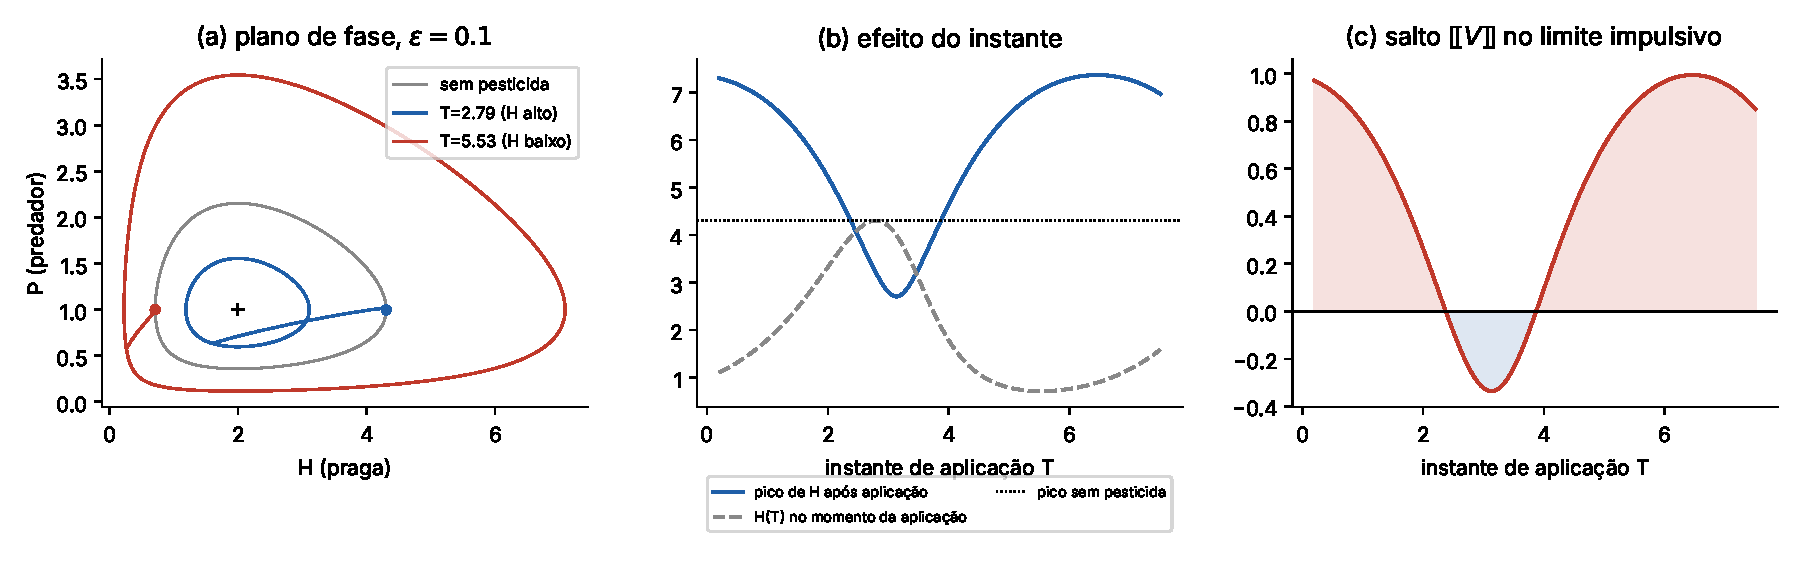
\includegraphics[width=\textwidth]{figuras/fig1_edo_instante.pdf}
\caption{Mecanismo local (sem difusão, $\omega=\Omega$), $\alpha_H=1$, $\alpha_P=0{,}5$.
(a) Aplicar com $H$ alto leva a um ciclo menor; com $H$ baixo, a um ciclo muito maior.
(b) Pico futuro em função do instante. (c) Salto \eqref{eq:saltoE}: pico maior $\iff\jump V>0$
(Proposição~\ref{prop:edo}).}
\label{fig:edo}
\end{figure}

\begin{figure}[ht]
\centering
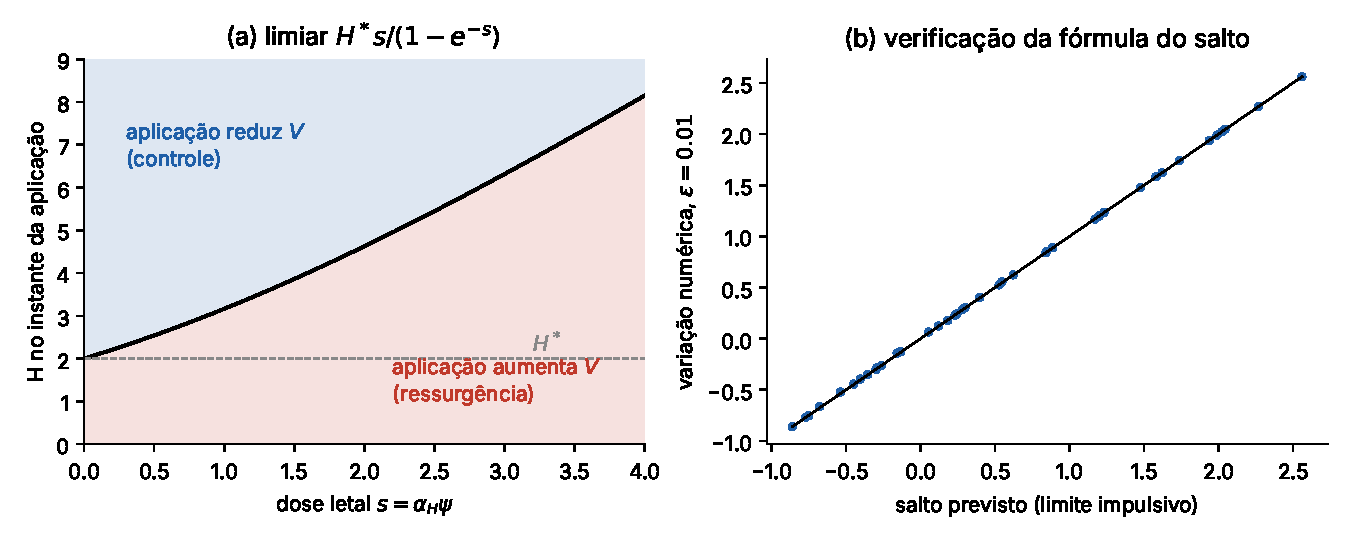
\includegraphics[width=0.85\textwidth]{figuras/fig2_limiar_dose.pdf}
\caption{(a) Limiar de dose do Corolário~\ref{cor:limiar} ($\alpha_P=0$), em termos de $\med H$.
(b) Verificação numérica da fórmula do salto com $\epsilon=0{,}01$.}
\label{fig:limiar}
\end{figure}

\begin{figure}[ht]
\centering
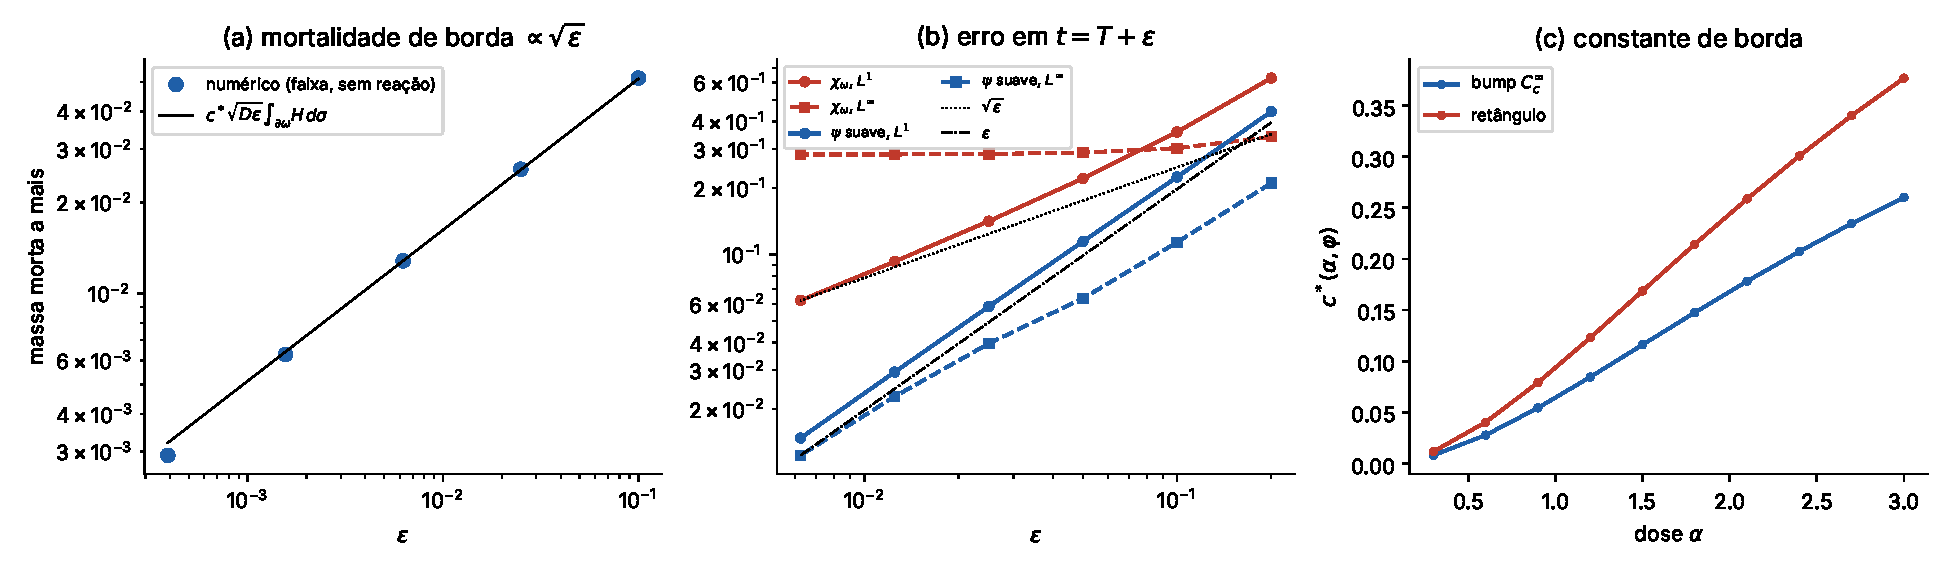
\includegraphics[width=\textwidth]{figuras/p3_convergencia_refugio.pdf}
\caption{O limite impulsivo com refúgio. (a) Problema linear numa faixa: a massa morta a mais em
relação ao limite impulsivo, medida em $t=T+5$, coincide com a previsão \eqref{eq:borda}
($2$ bordas, $h=4$, $c^*(1,\text{bump})=0{,}064$) e decai como $\sqrt\epsilon$.
(b) Modelo completo, erro em $t=T+\epsilon$. Com a borda nítida $\chi_\omega$: $L^1$ de ordem $1/2$
e $L^\infty$ que não decai (Proposição~\ref{prop:camada}). Com uma transição suave $\psi$: ordem $1$
nas duas normas. (c) Constante de borda $c^*(\alpha,\varphi)$ para o bump e para o retângulo de
\cite{LiYang}: o formato do pulso importa na ordem $\sqrt\epsilon$.}
\label{fig:conv}
\end{figure}

\begin{figure}[p]
\centering
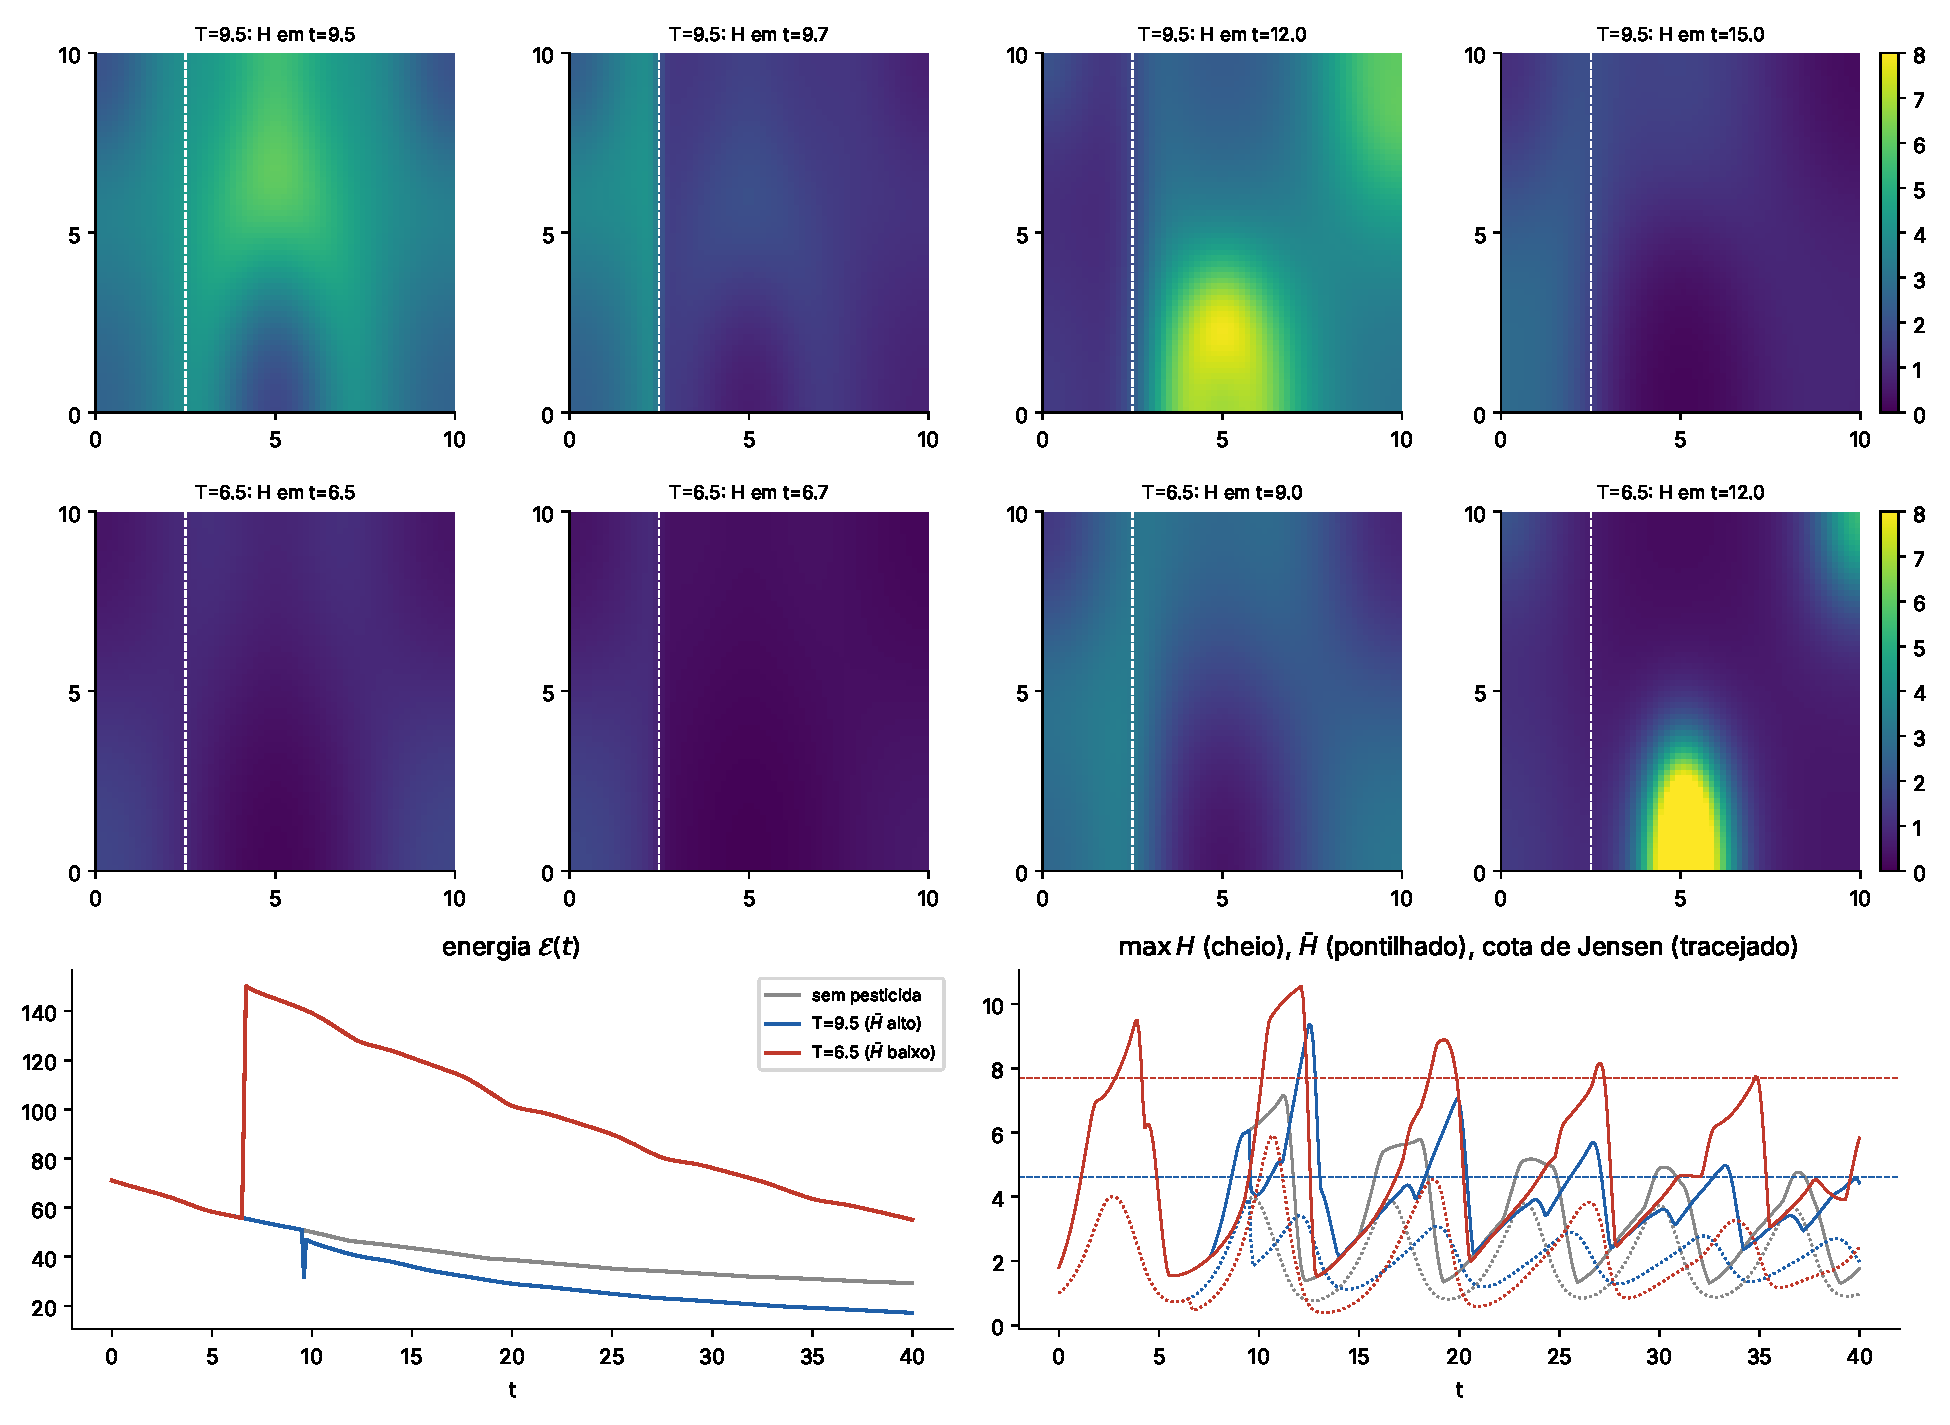
\includegraphics[width=\textwidth]{figuras/p4_planar_cenario.pdf}
\caption{Campo $\Omega=(0,10)^2$ com faixa de refúgio $\{x_1<2{,}5\}$ (à esquerda da linha
tracejada) e $\omega=\{x_1>2{,}5\}$; $\alpha_H=1{,}2$, $\alpha_P=0{,}6$, $\epsilon=0{,}2$.
Linha 1: aplicação com $\bar H$ alto. Linha 2: aplicação com $\bar H$ baixo. Linha 3: energia, pico e
média da praga, com a cota do Teorema~\ref{teo:cota} (tracejado). Com $T=9{,}5$, $\E$ cai de $51{,}2$ para $47{,}0$ e o pico de $\bar H$ cai de $3{,}98$ (sem pesticida) para $3{,}42$, mas o pico local sobe de $7{,}2$ para $9{,}4$ (Observação~\ref{obs:pico}). Com $T=6{,}5$, $\E$ salta de $56{,}0$ para $150{,}2$, $\bar H$ chega a $5{,}90$ e o pico local a $10{,}6$. Em ambos os casos $\bar H$ respeita a cota ($4{,}61$ e $7{,}70$).}
\label{fig:cenario}
\end{figure}

\begin{figure}[ht]
\centering
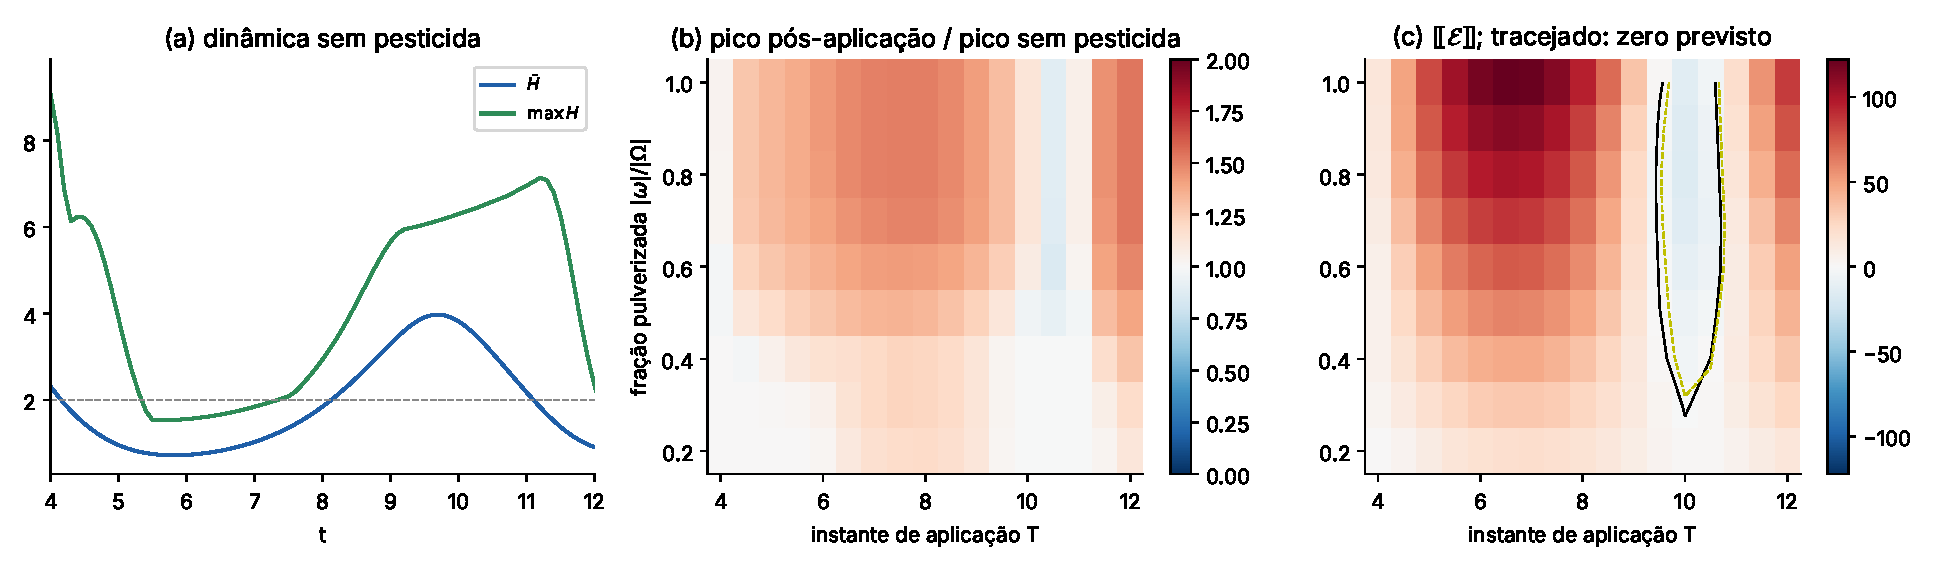
\includegraphics[width=\textwidth]{figuras/p5_refugio_instante.pdf}
\caption{Instante de aplicação $\times$ fração pulverizada, com o refúgio numa faixa
$\{x_1<x_r\}$ e $\epsilon=0{,}2$. (b) Razão entre o pico de $H$ após a aplicação e o pico sem pesticida.
(c) Salto de energia medido. A curva preta é o zero medido; a amarela tracejada é o zero previsto
por \eqref{eq:saltoE} com as médias em $\omega$ no instante $T$. A correlação entre o salto medido (com $\epsilon=0{,}2$) e o previsto pelas médias em $\omega$ é $0{,}996$, e as duas curvas de zero praticamente coincidem. A janela favorável é estreita ($T\approx9{,}5$--$10{,}5$, quando $\bar H$ está perto do máximo). Refúgios grandes (fração pequena) atenuam o efeito nos dois sentidos. Em (b) a razão fica entre $0{,}86$ e $1{,}54$: o pico \emph{local} raramente cai, de acordo com a Observação~\ref{obs:pico}.}
\label{fig:refugio}
\end{figure}

\begin{figure}[ht]
\centering
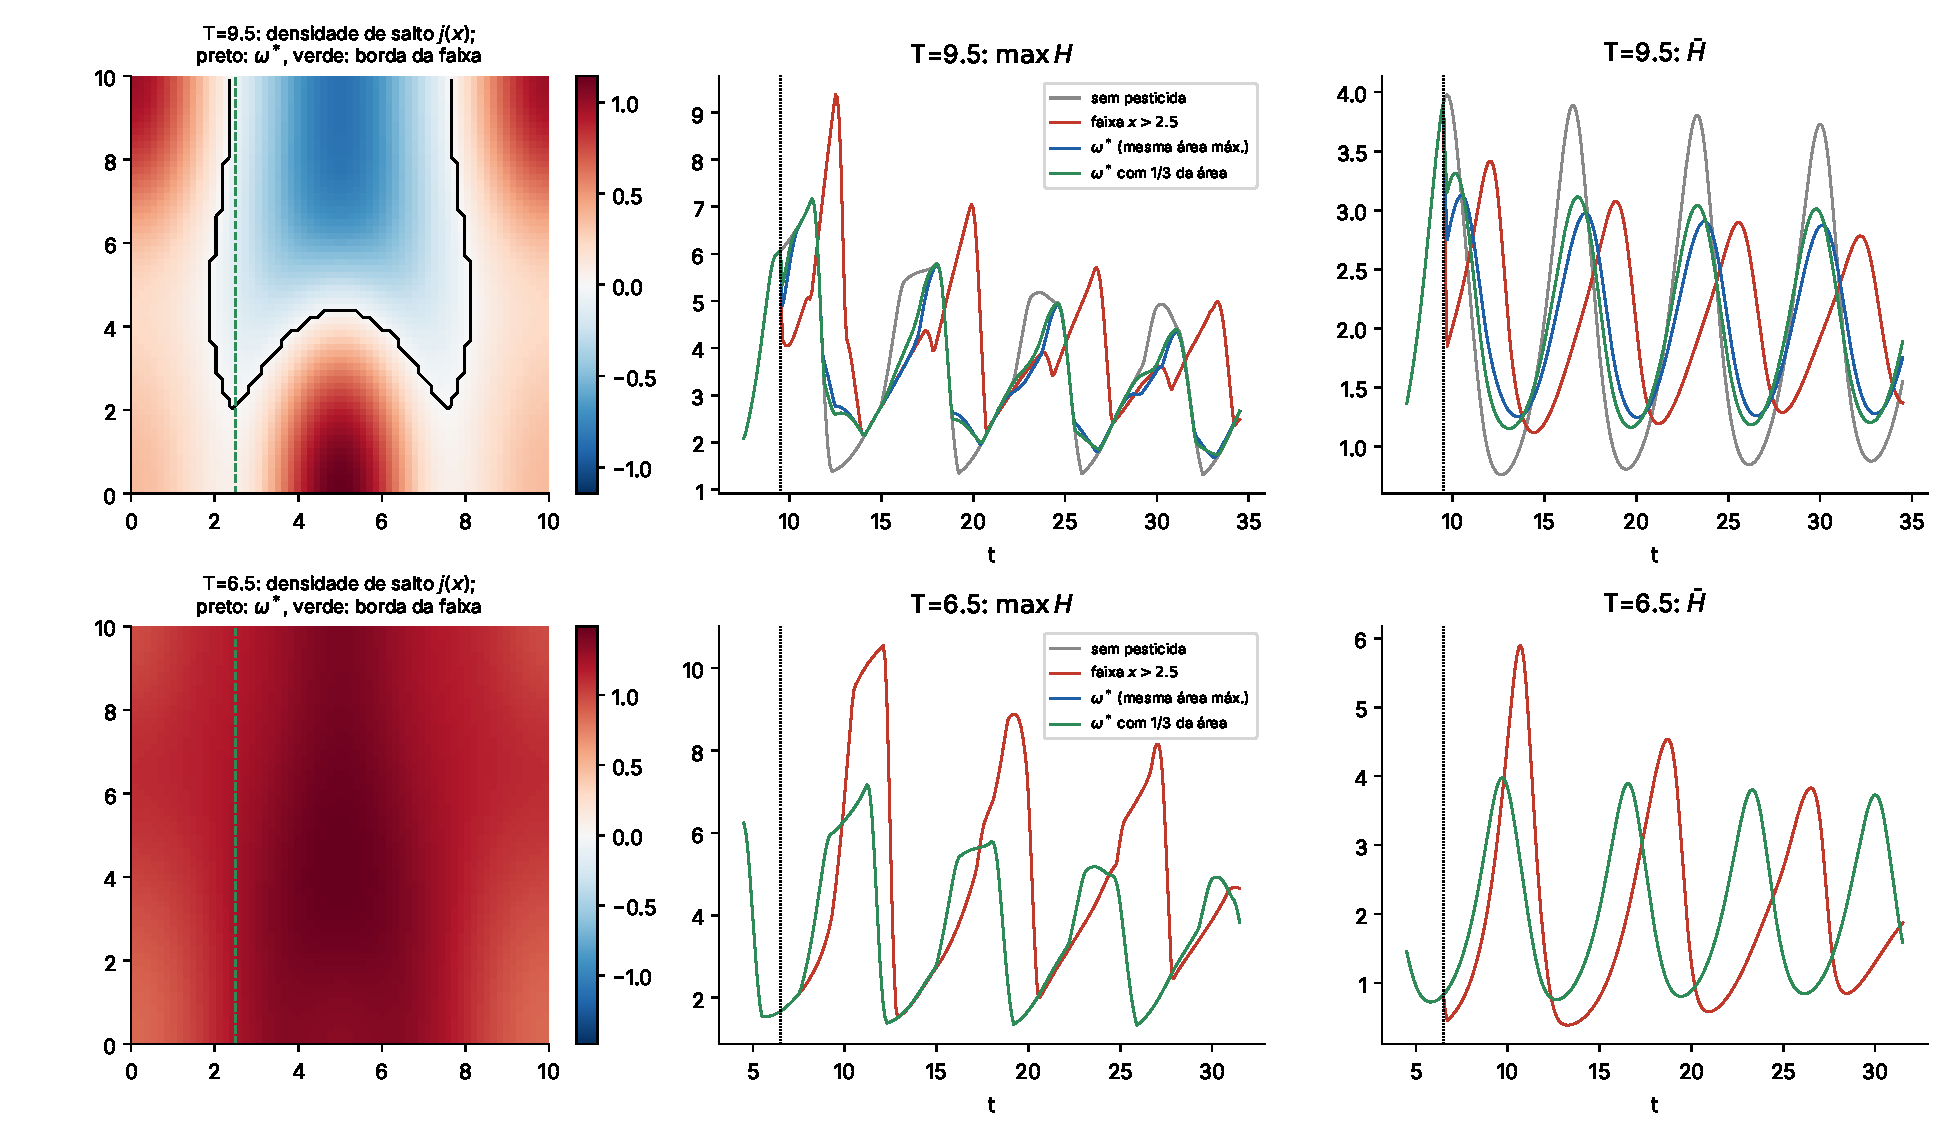
\includegraphics[width=\textwidth]{figuras/p6_zona_otima.pdf}
\caption{Zona ótima (Proposição~\ref{prop:banheira}) comparada com a faixa $\{x_1>2{,}5\}$ de mesma
área. Primeira coluna: densidade de salto $j$ em $T^-$; o contorno preto é $\omega^*$. Em $T=9{,}5$: $\{j<0\}$ ocupa $38\%$ do campo, e $\omega^*$ (área $38{,}3$, contra $75$ da faixa) dá $\jump{\E}=-17{,}2$, contra $-3{,}95$ da faixa. O pico local fica em $7{,}17$, igual ao sem pesticida, enquanto a faixa o eleva a $9{,}37$; o pico de $\bar H$ cai para $3{,}14$. Com só $1/3$ da área da faixa, $\jump{\E}=-14{,}8$. Em $T=6{,}5$: $j>0$ em todo o campo, logo $\omega^*=\emptyset$ (não aplicar), enquanto a faixa causa ressurgência ($\jump{\E}=+94{,}4$, $\bar H$ até $5{,}90$).}
\label{fig:otima}
\end{figure}

\begin{figure}[ht]
\centering
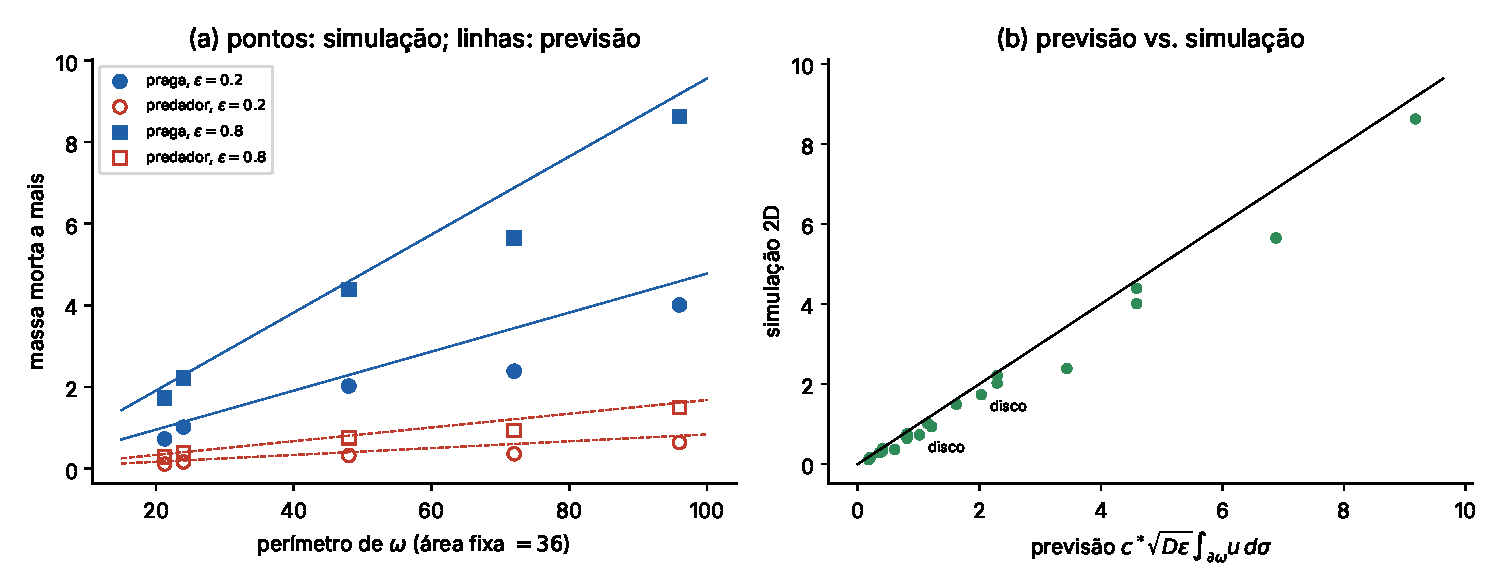
\includegraphics[width=0.85\textwidth]{figuras/p7_perimetro.pdf}
\caption{Mortalidade de borda no plano (Observação~\ref{obs:borda}). Problema linear (só difusão e
abate) com densidades uniformes $h=4$ (praga, $D_H=0{,}1$) e $p=1$ (predador, $D_P=0{,}05$), mesma dose
$\alpha=1{,}2$, área tratada fixa ($36$) dividida em $1$, $4$, $9$ ou $16$ quadrados ou num disco; malha
$160\times160$. (a) Massa morta a mais que no limite impulsivo em função do perímetro. (b) Simulação contra a
previsão $c^*\sqrt{D\epsilon}\,u\,\Per(\omega)$. Com a camada resolvida ($\epsilon=0{,}8$) e bordas
alinhadas à malha ($1$, $4$, $16$ quadrados), o erro fica entre $3$ e $6\%$; o resíduo vem dos cantos.
A razão predador/praga é $0{,}173$, contra $\sqrt{D_P/D_H}\,p/h=0{,}177$ previsto. Os desvios maiores
(disco, $9$ quadrados, $\epsilon=0{,}2$) ocorrem onde a malha suaviza a borda de $\omega$ ou não
resolve a camada $\sqrt{D\epsilon}$. Isso concorda com a teoria: uma transição suave reduz a mortalidade
de borda.}
\label{fig:perimetro}
\end{figure}

\clearpage
%======================================================================
\section{Discussão}

O refúgio entra no modelo pela função característica $\chi_\omega$, e isso tem duas
consequências de natureza diferente.

\emph{No limite impulsivo}, o refúgio só restringe o salto a $\omega$. Toda a teoria de energia se
mantém, e a decisão de aplicar depende das médias de $H$ e $P$ na zona tratada \eqref{eq:criterio}.
As duas conclusões de \cite{LiYang} viram enunciados precisos, e aparecem mais duas: o \emph{lugar}
importa (Corolário~\ref{cor:limiar}(iii)) e existe uma zona ótima explícita
(Proposição~\ref{prop:banheira}).

\emph{Para aplicações de duração finita}, a borda nítida do refúgio cria uma camada limite de
largura $\sqrt{D\epsilon}$. O limite impulsivo deixa de ser uniforme: a convergência é de ordem
$\sqrt\epsilon$ em $L^1$, com ordem ótima, contra $\epsilon$ para uma zona suave. A correção principal
tem significado biológico: uma mortalidade de borda proporcional ao perímetro de $\omega$, a
$\sqrt{D\epsilon}$ e a uma constante $c^*(\alpha,\varphi)$ que depende do formato do pulso. Ela atinge
mais a espécie mais móvel, o que dá um mecanismo espacial a mais para o paradoxo.

\paragraph{Problemas em aberto.} (1) Uma prova rigorosa da expansão da Observação~\ref{obs:borda}
para $\partial\omega$ curva, com o termo de curvatura; (2) o problema área--perímetro para
pulsos finitos; (3) os termos de taxia $\mp\nabla P\cdot\nabla H$ de \cite{LiYang}, que acrescentam a
\eqref{eq:identidade} a parcela sem sinal definido
$\int\nabla H\cdot\nabla P\,[c(1-\Hs/H)-(1-\Ps/P)]$; (4) a condição de Dirichlet; (5) aplicações
periódicas e o mapa de Poincaré impulsivo.

%======================================================================
\begin{thebibliography}{99}
\bibitem{LiYang} Y.~C.~Li, Y.~Yang, On the paradox of pesticides,
\emph{Commun.\ Nonlinear Sci.\ Numer.\ Simul.} 29 (2015) 179--187.
\bibitem{Hardin} M.~Hardin, B.~Benrey, M.~Coll, W.~Lamp, G.~Roderick, P.~Barbosa, Arthropod pest
resurgence: an overview of potential mechanisms, \emph{Crop Prot.} 14 (1995) 3--18.
\bibitem{Lester} P.~Lester, H.~Thistlewood, R.~Harmsen, The effects of refuge size and number on
acarine predator--prey dynamics in a pesticide-disturbed apple orchard, \emph{J.\ Appl.\ Ecol.} 35
(1998) 323--331.
\bibitem{Heong} K.~Heong, A.~Manza, J.~Catindig, S.~Villareal, T.~Jacobsen, Changes in pesticide use
and arthropod biodiversity in the IRRI research farm, \emph{Outlooks Pest Manage.} 18 (2007) 229--233.
\bibitem{AFP} L.~Ambrosio, N.~Fusco, D.~Pallara, \emph{Functions of Bounded Variation and Free
Discontinuity Problems}, Oxford Univ.\ Press, 2000.
\bibitem{EvansGariepy} L.~C.~Evans, R.~F.~Gariepy, \emph{Measure Theory and Fine Properties of
Functions}, CRC Press, 1992.
\bibitem{BrezisStrauss} H.~Brezis, W.~A.~Strauss, Semi-linear second-order elliptic equations in
$L^1$, \emph{J.\ Math.\ Soc.\ Japan} 25 (1973) 565--590.
\bibitem{Henry} D.~Henry, \emph{Geometric Theory of Semilinear Parabolic Equations}, Lecture Notes in
Math.\ 840, Springer, 1981.
\bibitem{Pazy} A.~Pazy, \emph{Semigroups of Linear Operators and Applications to Partial Differential
Equations}, Springer, 1983.
\bibitem{QS} P.~Quittner, Ph.~Souplet, \emph{Superlinear Parabolic Problems}, Birkhäuser, 2007.
\bibitem{Hale} J.~K.~Hale, \emph{Asymptotic Behavior of Dissipative Systems}, AMS, 1988.
\bibitem{LiebLoss} E.~H.~Lieb, M.~Loss, \emph{Analysis}, 2nd ed., AMS, 2001.
\bibitem{Lakshmikantham} V.~Lakshmikantham, D.~D.~Bainov, P.~S.~Simeonov, \emph{Theory of Impulsive
Differential Equations}, World Scientific, 1989.
\bibitem{Tang} S.~Tang, Y.~Xiao, L.~Chen, R.~A.~Cheke, Integrated pest management models and their
dynamical behaviour, \emph{Bull.\ Math.\ Biol.} 67 (2005) 115--135.
\end{thebibliography}

\end{document}
